\section{The \lhcb experiment}
\label{sec:lhcb}

\subsection{\lhc}
\label{sec:lhcb:lhc}

The Large Hadron Collider (\lhc) at the European Organization for Nuclear Research (\cern) is a particle accelerator designed to collide protons at a center-of-mass energy (\sqs) of 14\tev~\cite{lhc}. It has a peak design (instantaneous) luminosity of \lum$= 10^{34}\cm^{-2}\sec^{-1}$ for proton operation. It is also used to accelerate heavy ions. The accelerator complex at \cern is shown in Fig.~\ref{fig:lhc}. The four main experiments are \atlas, \cms, \lhcb and \alice. \atlas and \cms are both multipurpose experiments, while \alice is used for the study of heavy ion collisions. The present thesis concerns the \lhcb experiment, of which an overview of the goals and design of the experiment is given below.

\begin{figure}[!b]
\centering
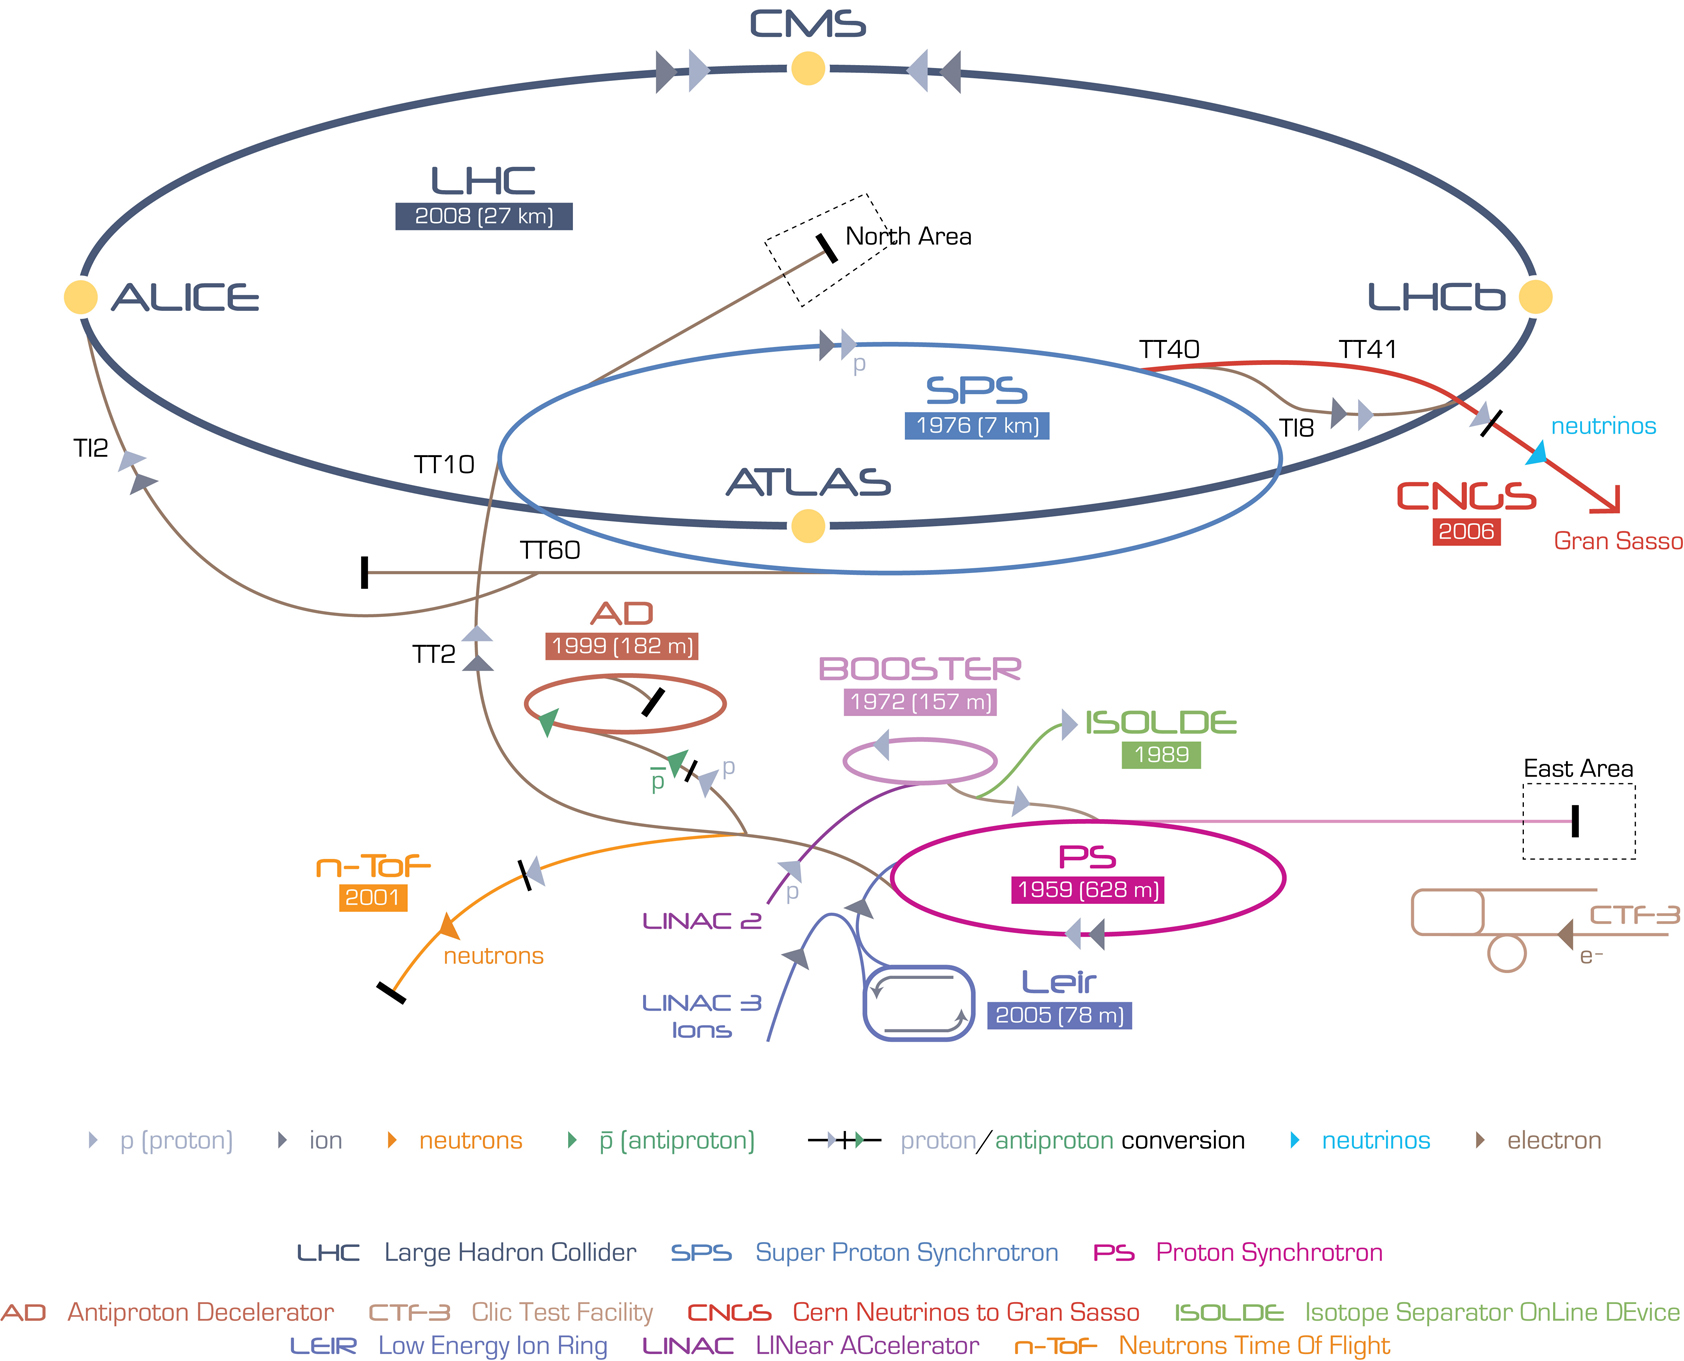
\includegraphics[width=\textwidth]{figs/detector/lhc.jpg}
\caption{Schematic view of the CERN accelerator complex.}
\label{fig:lhc}
\end{figure}

\subsection{\lhcb experiment}
\label{sec:lhcb:lhcb}

\lhcb is a dedicated heavy flavour experiment with the primary goal of searching for indirect evidence of NP in \CP violation and rare decays of beauty and charm hadrons~\cite{lhcb}. Due to the large beauty and charm production cross-sections provided by the \lhc, the \lhcb experiment was able to collect $\sim$10$^{12}$ heavy flavour decays during data taking in 2011 and 2012~\cite{lhcb-perf}.

The data used for physics analysis in this thesis was collected in 2011 and 2012. In 2011, the center-of-mass energy was 7\tev and the majority of the data was taken at a instantaneous luminosity of $3.5\times10^{32}\cm^{-2}\sec^{-1}$. In 2012, the center-of-mass energy was increased to 8\tev and the data was taken at a instantaneous luminosity of $4\times10^{32}\cm^{-2}\sec^{-1}$. This corresponds to an integrated luminosity of 1.11\invfb in 2011 and 2.08\invfb in 2012.

The \lhcb detector is a single arm forward spectrometer that covers a pseudo-rapidity range of $2 < \eta < 5$. The layout of the \lhcb detector, shown schematically in Fig.~\ref{fig:lhcb-run1}, is motivated by the physics of \bquark quark production at the \lhc. The dominant production processes for \bquark\bquarkbar pairs in \proton\proton collisions are gluon-gluon fusion and quark-antiquark annihilation, as illustrated in Fig.~\ref{fig:b-production}. In the high energy collisions present at the \lhc, the \bquark\bquarkbar pairs tend to be produced in the same forward or backward cone, shown in Fig.~\ref{fig:b_bbar_correlation}.  Therefore, due to its unique geometry, \lhcb is able to detect $\sim40\%$ of the heavy quark pairs despite only covering only $\sim4\%$ of the total solid angle.

The following requirements are crucial in order to fulfil the \lhcb physics programme: efficient, robust and flexible triggering on a variety of different final states, excellent tracking (momentum, impact parameter (IP) and primary vertex (PV) resolution), precise decay time resolution and excellent particle identification.

\begin{sidewaysfigure}
\centering
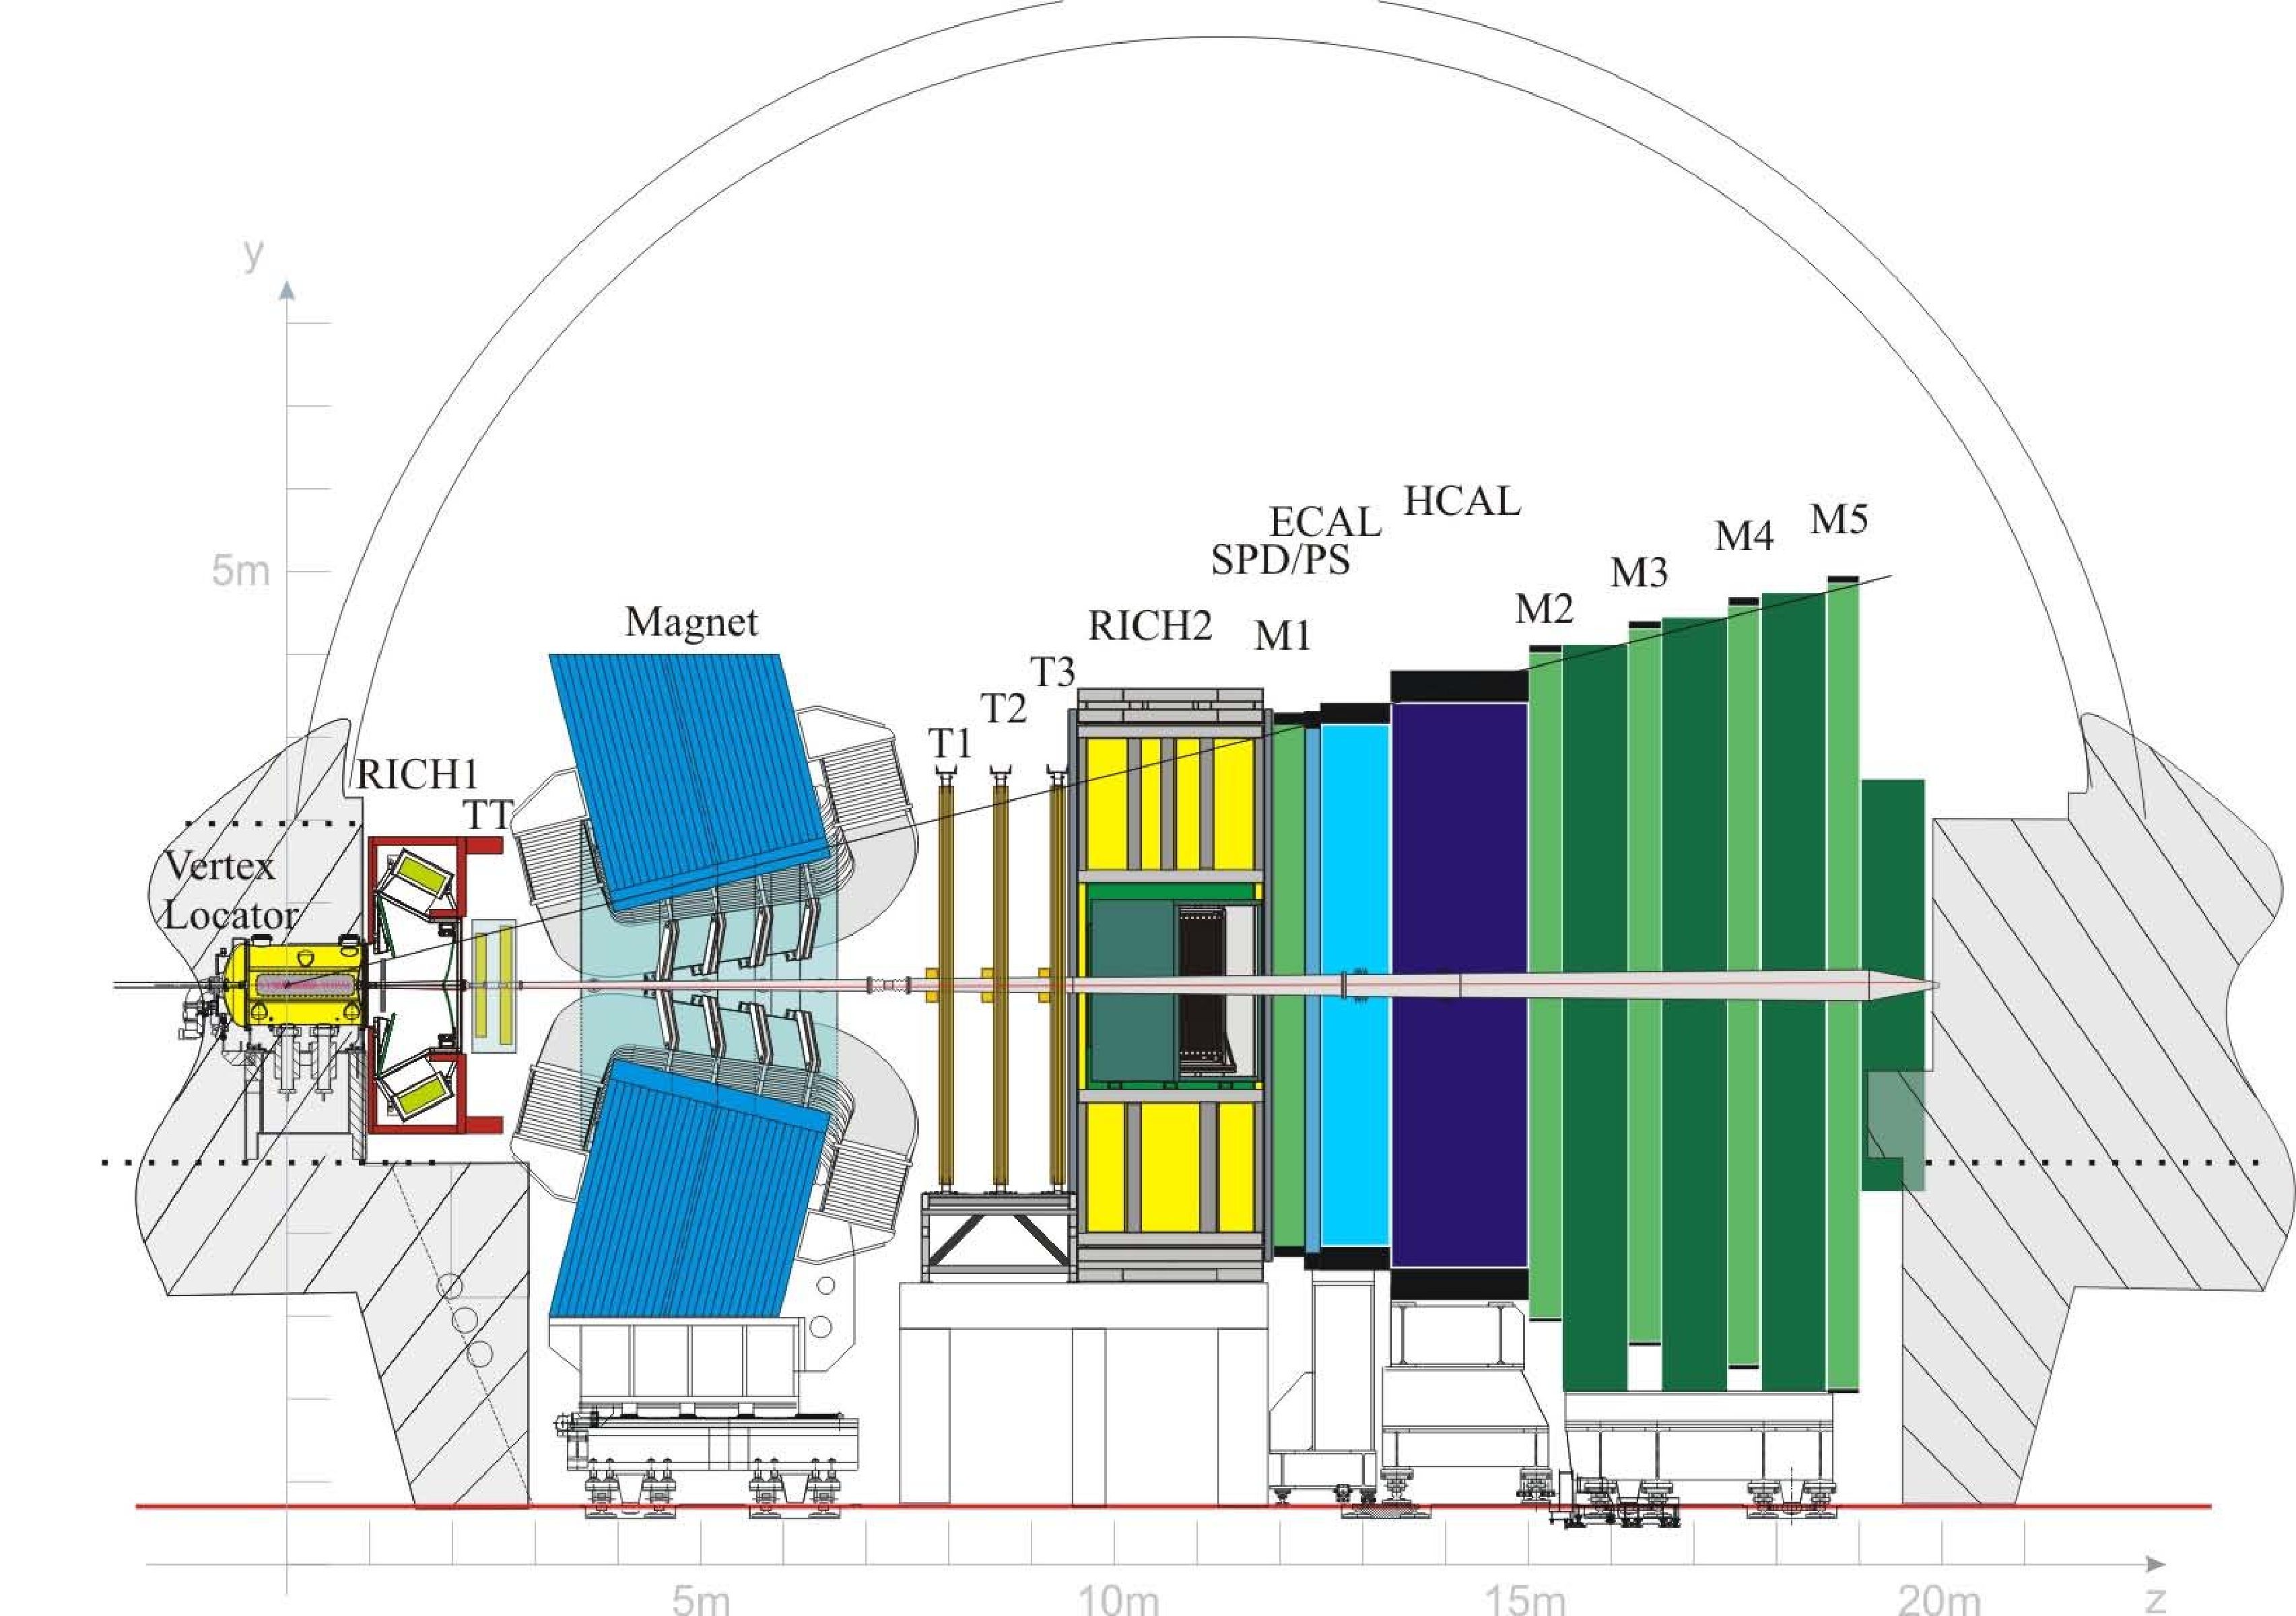
\includegraphics[width=0.9\textwidth]{figs/detector/lhcb-run1.pdf}
\caption{Schematic view of the \lhcb detector.}
\label{fig:lhcb-run1}
\end{sidewaysfigure}

\begin{figure}[!tb]
\centering
\begin{subfigure}{0.4\textwidth}
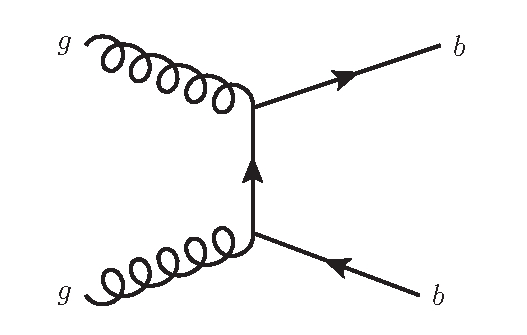
\includegraphics[width=\linewidth]{figs/detector/gluon_fusion.eps}
\caption{}
\label{fig:b-production:a}
\end{subfigure}
\begin{subfigure}{0.4\textwidth}
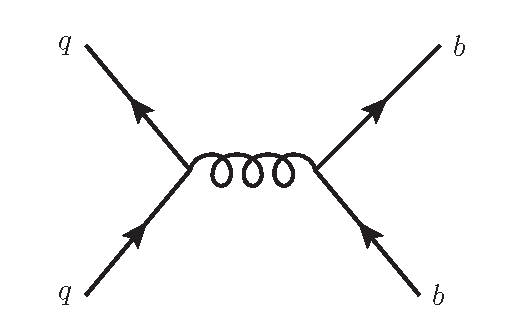
\includegraphics[width=\linewidth]{figs/detector/quark_antiquark_annihilation.eps}
\caption{}
\label{fig:b-production:b}
\end{subfigure}
\caption{Feynman diagrams of the dominant production processes for \bquark\bquarkbar pairs in proton-proton collisions. These are (a) gluon-gluon fusion and (b) quark-antiquark annihilation~\cite{b-production}.}
\label{fig:b-production}
\end{figure}

\begin{figure}[!tb]
\centering
\includegraphics[width=0.5\textwidth]{figs/detector/b_bbar_correlation.pdf}
\caption{The angular distribution of \bquark\bquarkbar pairs in terms of the polar angle from the beam axis. The red area shows the acceptance of the \lhcb detector.}
\label{fig:b_bbar_correlation}
\end{figure}


\subsubsection{Dipole magnet}

A warm dipole magnet~\cite{magnet-tdr} is used in order to allow a measurement of the momentum of charged particles in the forward acceptance of $\pm$250\mrad vertically and $\pm$300\mrad horizontally. It provides an integrated magnetic field of 4~Tm for tracks of 10\m in length. The strength of the main component of the magnetic field, $B_{y}$, as a function of $z$ is shown in Fig.~\ref{fig:magnet}. The location of the tracking sub-detectors, described in Sec.~\ref{sec:lhcb:tracking}, are also shown. The polarity of the magnetic field is changed regularly in order to be able to control possible detection asymmetries.

\begin{figure}[!tb]
\centering
\adjincludegraphics[width=\textwidth,trim={{.1\width} {.62\height} {.1\width} {.1\height}},clip]{figs/detector/magnet.pdf}
\caption{The strength of the main component of the magnetic field, $B_{y}$, as a function of $z$. The location of the tracking sub-detectors are shown.}
\label{fig:magnet}
\end{figure}

\subsubsection{Tracking system}
\label{sec:lhcb:tracking}

The trajectory of charged particles traversing the \lhcb detector are reconstructed using a dedicated tracking system. The tracking system consists of a high granularity vertex detector surrounding the \proton\proton interaction region, a large area silicon-strip detector located upstream of the magnet, and three stations of silicon-strip detectors and straw drift tubes placed downstream of the magnet. By determining the deflection of the charged particles that have passed through the magnetic field their momentum can be measured.

The Vertex Locator (\velo)~\cite{velo-tdr,velo-perf} is a silicon microstrip detector that provides measurements of track coordinates close to the \proton\proton interaction region. These precision measurements are used to identify both the primary interaction vertices and the displaced secondary vertices of the decays of \bquark and \cquark hadrons. The detector consists of 42 silicon micro-strip stations with $r$-$\phi$ geometry, shown schematically in Fig.~\ref{fig:velo}. It has two retractable halves which are opened and closed during each \lhc fill. When closed, the sensors are positioned only 7\mm from the \lhc beam. This is essential in achieving precise IP measurements.

\begin{figure}[!tb]
\centering
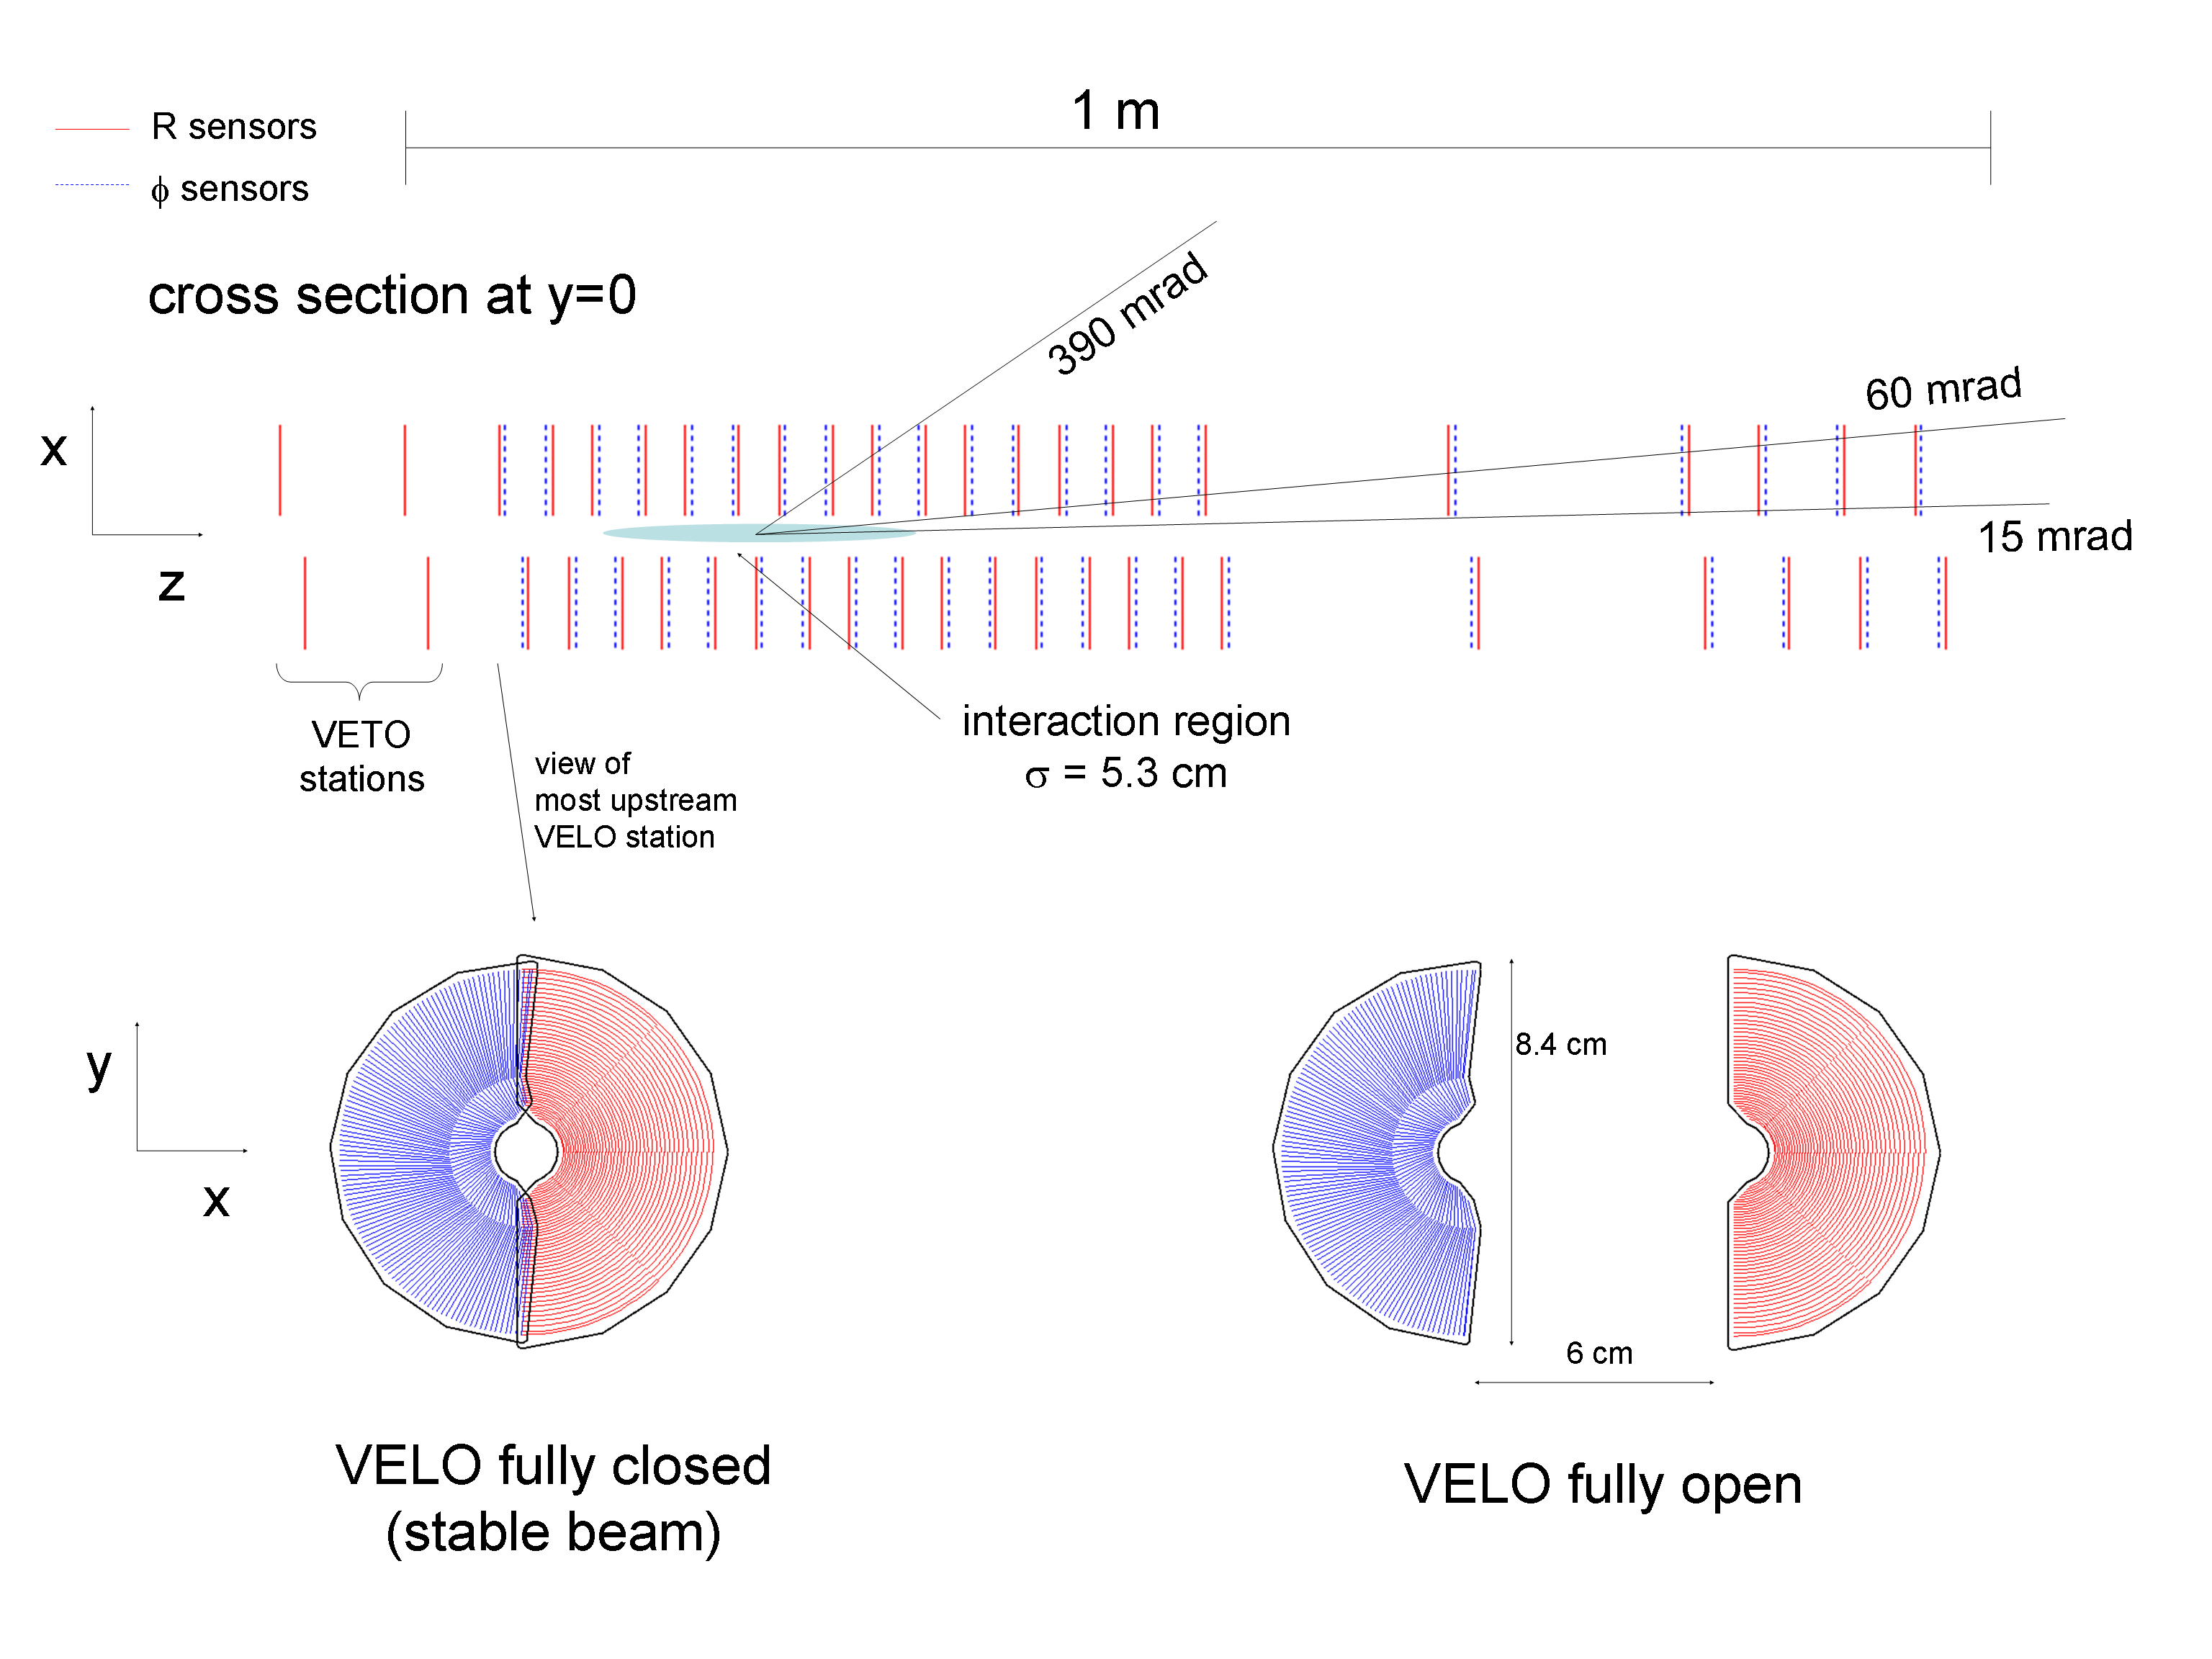
\includegraphics[width=\textwidth]{figs/detector/velo.png}
\caption{Schematic view of the \velo detector.}
\label{fig:velo}
\end{figure}

The Silicon Tracker (ST) consists of two silicon microstrip detectors: the Tracker Turicensis\footnote{Formerly known as the Trigger Tracker.} (TT)~\cite{lhcb-tdr} and the Inner Tracker (IT)~\cite{it-tdr}. The TT is located upstream of the magnet and covers the full acceptance of the experiment. The IT is located downstream of the magnet and covers a cross-shaped region at the center of the three tracking stations. Each ST station contains four layers with a \mbox{$x$-$u$-$v$-$x$} layout such that the $u$ and $v$ layers are tilted by $\pm$ 5$^{\circ}$ with respect to the vertical. The inclined layers allow stereo measurements to be made. A schematic view of the TT sub-detector is shown in Fig.~\ref{fig:tt}. As the beampipe passes through the TT there is a square hole at the center of the detector which reduces its acceptance. The square hole has a width of 7.7\cm at the first TT sub-station (TTa) and 8.0\cm at the second (TTb).

\begin{figure}[!tb]
\centering
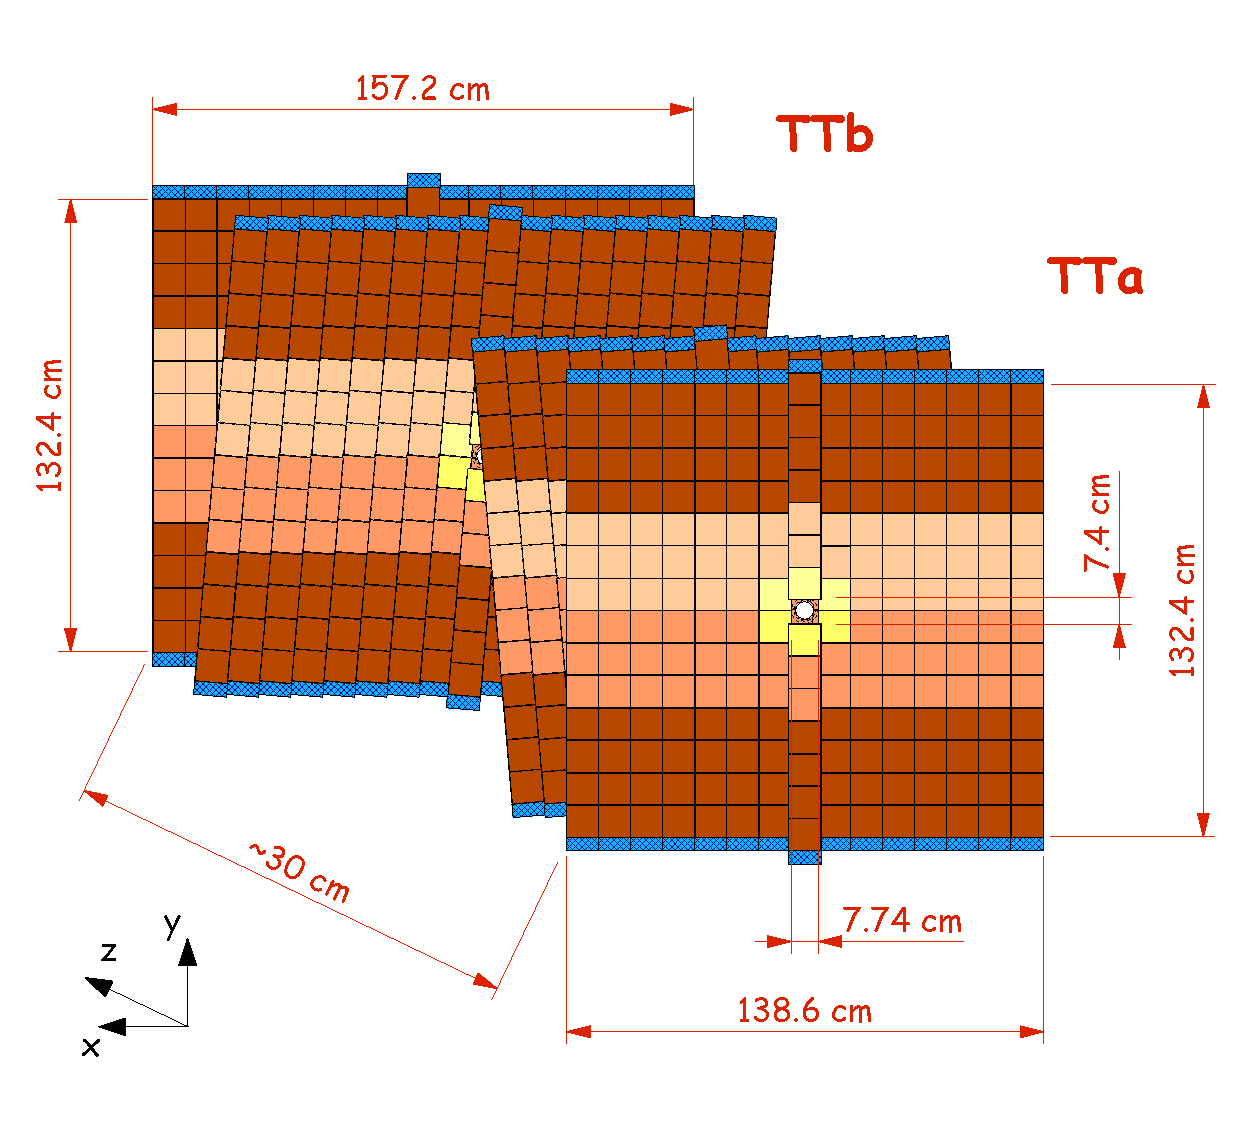
\includegraphics[width=0.8\textwidth]{figs/detector/tt.pdf}
\caption{Schematic view of the TT sub-detector geometry. The different colours indicate the number of sensors that are wire bonded together in the $y$ direction.}
\label{fig:tt}
\end{figure}

The Outer Tracker (OT)~\cite{ot-tdr,ot-perf} is a drift-time detector made up of arrays of individual straw-tube modules. The modules each contain two staggered layers of drift-tubes of 4.9\mm in diameter. They are filled with a mixture of Argon (70\%) and \cotwo (30\%), which provides both fast drift times and sufficient drift-coordinate resolution. The detector consists of three stations each with four layers arranged with a \mbox{$x$-$u$-$v$-$x$} layout such that the $u$ and $v$ layers are tilted by $\pm$ 5$^{\circ}$ with respect to the vertical.

The track reconstruction efficiency can be defined as the probability that the trajectory of a charged particle that has passed through the full tracking system is reconstructed. This can be measured in data using a tag-and-probe method with \decay{\jpsi}{\mumu} decays \cite{tracking-perf}. One of the daughters is fully reconstructed (tag), while the other is only partially (probe), although well enough to reconstruct the $J/\psi$ invariant mass.  The efficiency can then be measured by matching the probe track to a fully reconstructed track. The average efficiency is found to be over 95\% and is only slightly affected in high multiplicity events.

The momentum resolution for tracks passing through the full tracking system can be measured in data using \decay{\jpsi}{\mumu} decays \cite{lhcb-perf}. The relative momentum resolution, $\delta p/p$ is found to be between 0.4\% - 0.6\% for tracks up to 100\gevc. The mass resolution is determined from data by studying the \jpsi, \psitwos, $\Upsilon$ and \Z resonances. The relative mass resolution, $\sigma_{m}/m$, is found to be about 5 per mille up to the $\Upsilon$ masses.

Precise vertex resolution is important to allow the separation of primary and secondary decay vertices. The primary vertex resolution depends strongly on the number of tracks used to form it. It can be measured in data in an event-by-event manner by randomly splitting the track sample in two and reconstructing the PV using each independent set of tracks. In 2011 data, a 25-track vertex was found to have a resolution of 13\mum in $x$ and $y$ and 71\mum in $z$~\cite{lhcb-perf}.
 
While the reconstructed decay time of charm and beauty hadrons is used in offline selections and for precise measurements of lifetimes, the most stringent requirement on the decay time resolution originates from the need to resolve the fast \Bs-\Bsb oscillations in mixing. The decay time resolution is topology dependent and is calibrated in data for each final state using prompt combinations that fake the signal candidates. The shape of the prompt decay time distribution is determined only by the resolution function. The typical decay time resolution is 45\fs for a 4-track vertex~\cite{lhcb-perf}.

\subsubsection{Particle identification}
\label{sec:lhcb:pid}

Excellent particle identification (PID) is a crucial requirement for \lhcb. Charged particle identfication is important to be able distinguish specific final states from those with otherwise identical topologies and to perform \bquark quark flavour tagging. Detecting photons is essential to allow the reconstruction of rare radiative decays. As muons are present in the final state of many \CP-sensitive states such as \BsToJPsiPhi and rare modes such as \BsToMuMu their triggering and identification are of fundamental importance.

The primary goal of the \rich system~\cite{lhcb-tdr,rich-perf} is the identification of charged hadrons (\pion, \kaon, \proton). This is achieved by exploiting the Cherenkov effect by which a charged particle travelling in a medium will emit Cherenkov radiation whenever the velocity of the particle exceeds the velocity of light in that medium. The cone of light will be emitted at a particular angle ($\theta_{c}$) relative to the particle path. \rich detectors use a combination of spherical and flat mirrors to focus the cone of light into a ring. This ring is then projected onto an array of photodetectors. The Cherenkov angle ($\theta_{c}$) can be determined from the radius of the ring. The velocity of the particle is found from $\theta_{c}$\footnote{$\cos\theta_{c} = \frac{1}{n\beta}$ where $\beta = \frac{v}{c}$ and $n$ is the refractive index of the medium}. Combining this velocity with the momentum measured by the tracking systems allows the determination of the particle mass and, therefore, the type of particle. 

In the forward region covered by \lhcb, there is a strong anticorrelation between polar angle and momentum. Due to this, the \rich system consists of two detectors. The detector upstream of the magnet, \richone, covers the low and intermediate momentum region 2-40\gevc for the full angular acceptance 15-300\mrad. The downstream detector, \richtwo, covers the high momentum region 15-100\gevc over a reduced angular acceptance 15-120\mrad. \richone contains aerogel and \cfourften as gas radiators while \richtwo contains \cffour. The relationship between Cherekov angle and particle momentum is shown in Fig.~\ref{fig:radiators} for each of the three radiators.

\begin{figure}[!tb]
\centering
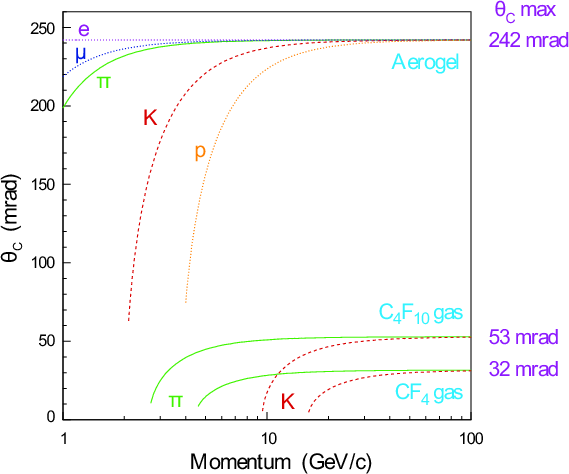
\includegraphics[height=0.3\textheight]{figs/detector/radiators.png}
\caption{Cherenkov angle versus particle momentum for the three gas radiators used in the \rich system.}
\label{fig:radiators}
\end{figure}

The calorimeter system~\cite{calo-tdr} is used both to identify and to measure the position and energy of photons, electrons and hadrons. It consists of a Scintillating Pad Detector (SPD), a Preshower (PS), an electromagnetic calorimeter (ECAL) and a hadronic calorimeter (HCAL). The ECAL is scintillator/lead sampling calorimeter with an energy resolution of $\sigma_{E}/\sqrt{E} = 1\% + 10\%/\sqrt{E}$. The HCAL is scintillator/iron sampling calorimeter with an energy resolution of approximately $\sigma_{E}/\sqrt{E} \sim 70\%/\sqrt{E}$. 

The muon system~\cite{muon-tdr,muon-tdr2,muon-tdr3,muon-perf} is used to identify muons and consists of five stations. The first station, M1, is located upstream of the calorimeters and uses triple Gas Electron Multiplier (GEM) detectors. The remaining four stations, M2-M5, located downstream of the calorimeters use Multiwire Proportional Chambers (MWPC) which are interleaved with 80\cm thick iron absorbers to select penetrating muons.

For a given particle hypothesis (\kaon, \pion, \muon, \proton), a combined, overall likelihood is obtained using information from the \rich detectors, the calorimeters and the muon system. The variable commonly used for PID selection requirements is the delta log likelihood (\dll), for example,

\begin{equation}
\dllkpi = \log(\lum_{\kaon}) - \log(\lum_{\pion})
\end{equation}

\noindent where $\lum_{\kaon}$ is the likelihood that the particle is a kaon and $\lum_{\pion}$ is the likelihood that the particle is a pion.
\subsubsection{Trigger system}
\label{detector:trigger}

The \lhcb trigger system~\cite{trigger-tdr,trigger-perf} plays an important role in selecting signal events and rejecting background. Two key signatures of the decays of beauty and charm hadrons are large invariant masses and large lifetimes, with respect to light unflavoured particles. The large invariant masses result in the daughter particles having significant transverse momentum with respect to the beam axis (\pt). The large lifetimes lead to the daughter particles having a large IP with respect to the primary vertex. Several key channels also contain muons in the final state.

The trigger system consists of two stages: a hardware trigger (\lone) followed by a high-level trigger implemented in software (\hlt). The trigger scheme used in 2012 data taking is shown in Fig.~\ref{fig:trigger:runI}. The task of the L0 trigger is to reduce the event rate from the rate of visible interactions at $\sim$13\mhz to 1\mhz at which the \lhcb detector can be read out. Therefore, a decision based on information from the muon systems and calorimeters needs to be reached in less than 4\mus. Events that contain high \pt muons or large transverse energy deposits in either calorimeter are selected by L0.

In the first stage of the software trigger (\hltone), a partial event reconstruction is performed due to the limitations of the available computing power. In order to reduce the time taken, only \velo track segments that either have a large IP with respect to the primary vertex or are matched to hits in the muon stations are extrapolated into the main tracking system.\footnote{The IP requirements bias the observable lifetime distributions for fully hadronic \bquark hadron decays.} The event is selected if a good quality track with a large \pt is found, further reducing the event rate to 70\khz. 

Events selected by \hltone are passed to the second stage of the software trigger (\hlttwo). In this stage, all tracks with a minimum \pt greater than 300\mevc are reconstructed without any requirement on IP or matched muon hits. A combination of exclusive and inclusive selections are used to reduce the event rate to 5\khz, which is written to disk. The inclusive selection of heavy flavour decays with hadrons in the final state is performed by a ``topological'' algorithm containing a multivariate classifier that identifies \bquark hadron decays with two-, three- and four-track vertices~\cite{trigger-inclusive,trigger-topo}.

\begin{figure}[!tb]
\begin{subfigure}{0.49\textwidth}
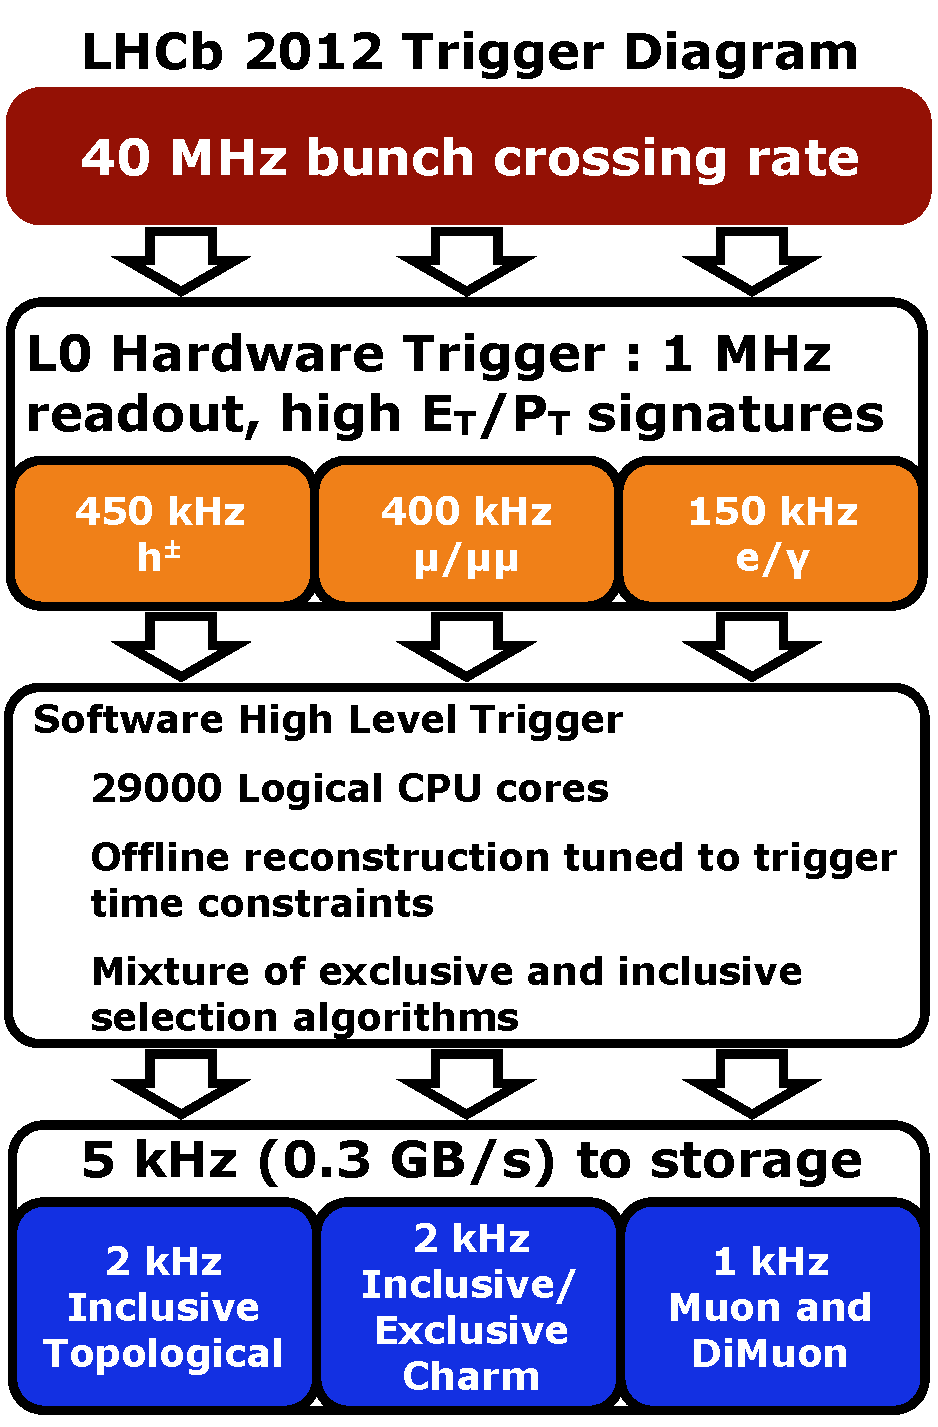
\includegraphics[width=0.9\textwidth]{figs/detector/trigger-runI.pdf}
\caption{}
\label{fig:trigger:runI}
\end{subfigure}
\begin{subfigure}{0.49\textwidth}
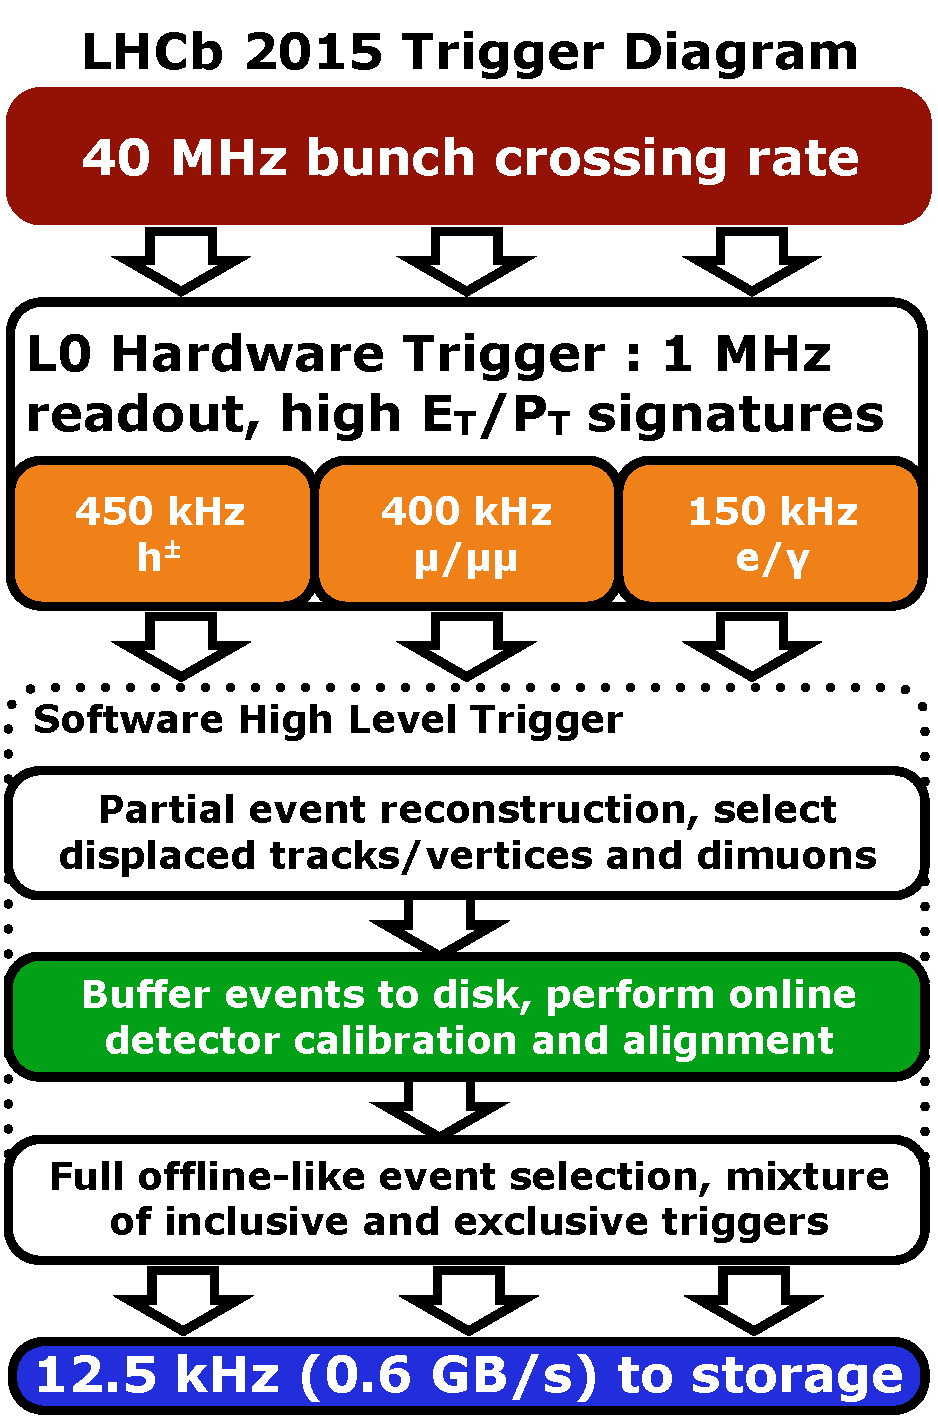
\includegraphics[width=0.9\textwidth]{figs/detector/trigger-runII.pdf}
\caption{}
\label{fig:trigger:runII}
\end{subfigure}
\caption{The trigger schemes used for (a) 2012 and (b) 2015 data taking.}
\label{fig:trigger}
\end{figure}

\subsection{\lhcb Run II}
\label{sec:lhcb:lhcb-run2}

During Run II of the \lhc (2015-2018), the \lhcb experiment will take data at an increased center-of-mass energy of \sqs = 13\tev. The bunch spacing will change from 50\ns to the design value of 25\ns. With these conditions the same instantaneous luminosity of $4\times10^{32}\cm^{-2}\sec^{-1}$ as for 2012 data taking can be achieved with a lower pile-up. 

The software trigger used in Run I contained only a simplified track reconstruction sequence with respect to the sequence used in the full offline event reconstruction. Furthermore, only a preliminary alignment and calibration of the detector was available and no information from the \rich system was used. For Run II, the trigger system was redesigned with two key objectives: to enable the full offline event reconstruction to be performed within the trigger and to achieve the same alignment and calibration quality at the trigger level as could be achieved offline during Run I~\cite{hlt-runII}. These two features allow physics analyses to be performed directly on the output of the software trigger~\cite{turbo}.

The trigger scheme used in 2015 data taking is shown in Fig.~\ref{fig:trigger:runII}. Following the hardware stage and a partial event reconstruction, selected events are buffered to disk. The automatic alignment and calibration procedure is then performed~\cite{alignment}. Once the detector is aligned and calibrated the full offline event reconstruction is performed. With the full information available, including PID from the \rich system, a wide range of inclusive and exclusive selections can be performed in order to trigger the event.

 Under the new trigger scheme it is also possible to only write out the information of the signal candidates~\cite{turbo}. This leads to a large saving in storage space ($\sim 90$\%) and is ideal for the analysis of channels with high yields that would previously have been heavily pre-scaled. It also allows rapid turn-around from data taking to analysis on the order of a few weeks~\cite{jpsi-em,charm-em}. However, this trigger scheme requires careful planning of the selection criteria in order to not leave out potential interesting physics cases.

\subsection{\lhcb Upgrade}
\label{sec:lhcb:lhcb-upgrade}

The \lhcb experiment will undergo an upgrade during Long Shutdown 2 (2018-2019) to allow data taking at \sqs = 14\tev with an instantaneous luminosity of $2\times10^{33}$cm$^{-2}$s$^{-1}$~\cite{upgrade-loi,upgrade-tdr}. The upgraded detector will collect at least 50\invfb of integrated luminosity in 10 years of operation.

Two key features of the \lhcb Upgrade are the following: a trigger-less readout system and a full software trigger~\cite{upgrade-trigger-tdr}. With the current experiment the collision rate must be reduced to the readout rate of 1\mhz. This is achieved using basic information from the calorimeters and muon system as described in Sec.~\ref{detector:trigger}. The largest inefficiencies in the trigger chain, especially for purely hadronic decays, occur at this stage. Furthermore, this constraint inhibits the operation of the detector at higher instantaneous luminosities as trigger yields for hadronic channels would saturate, as shown in Fig.~\ref{fig:upgrade-motivation}. Removing this bottleneck, by implementing a trigger-less readout system will allow the full rate of visible interactions to be processed by a purely software trigger. This trigger will offer great flexibility and improve the trigger efficiency significantly for a number of physics channels. It will also allow lifetime unbiased hadronic triggering for the first time at a hadron collider.

\begin{figure}[!tb]
\centering
\adjincludegraphics[width=0.8\textwidth,trim={{.2\width} {.59\height} {.2\width} {.1\height}},clip]{figs/detector/upgrade-motivation.pdf}
\caption{The trigger yield as a function of instantaneous luminosity for different decays of \B mesons~\cite{upgrade-loi}.}
\label{fig:upgrade-motivation}
\end{figure}

In order to incorporate a trigger-less readout, all the front-end electronics need to be replaced. Futhermore, the upgraded detector will need to be able to cope with the factor five increase in instantaneous luminosity. Therefore, many of the existing sub-detectors will be replaced. The current \velo will be replaced by the \velo Pixel (VP) detector~\cite{upgrade-velo-tdr}. The VP will contain 41 million $55\times55$\mum pixel sensors with micro-channel \cotwo cooling. When closed, the first pixel will be located just 5.1\mm from the \lhcb beam. The TT will be replaced by the Upstream Tracker (UT), shown schematically in Fig.~\ref{fig:ut}~\cite{upgrade-tracker-tdr}. The UT will be a high granularity silicon microstrip detector with improved coverage of the \lhcb acceptance. The IT and OT will be replaced by the Scintillating Fibre Tracker (SciFi)~\cite{upgrade-tracker-tdr}. This single, fast detector will contain 2.5\m long multilayer ribbons of 250\mum diameter scintillating fibres with silicon photomultiplier readout.

\begin{figure}[!tb]
\centering
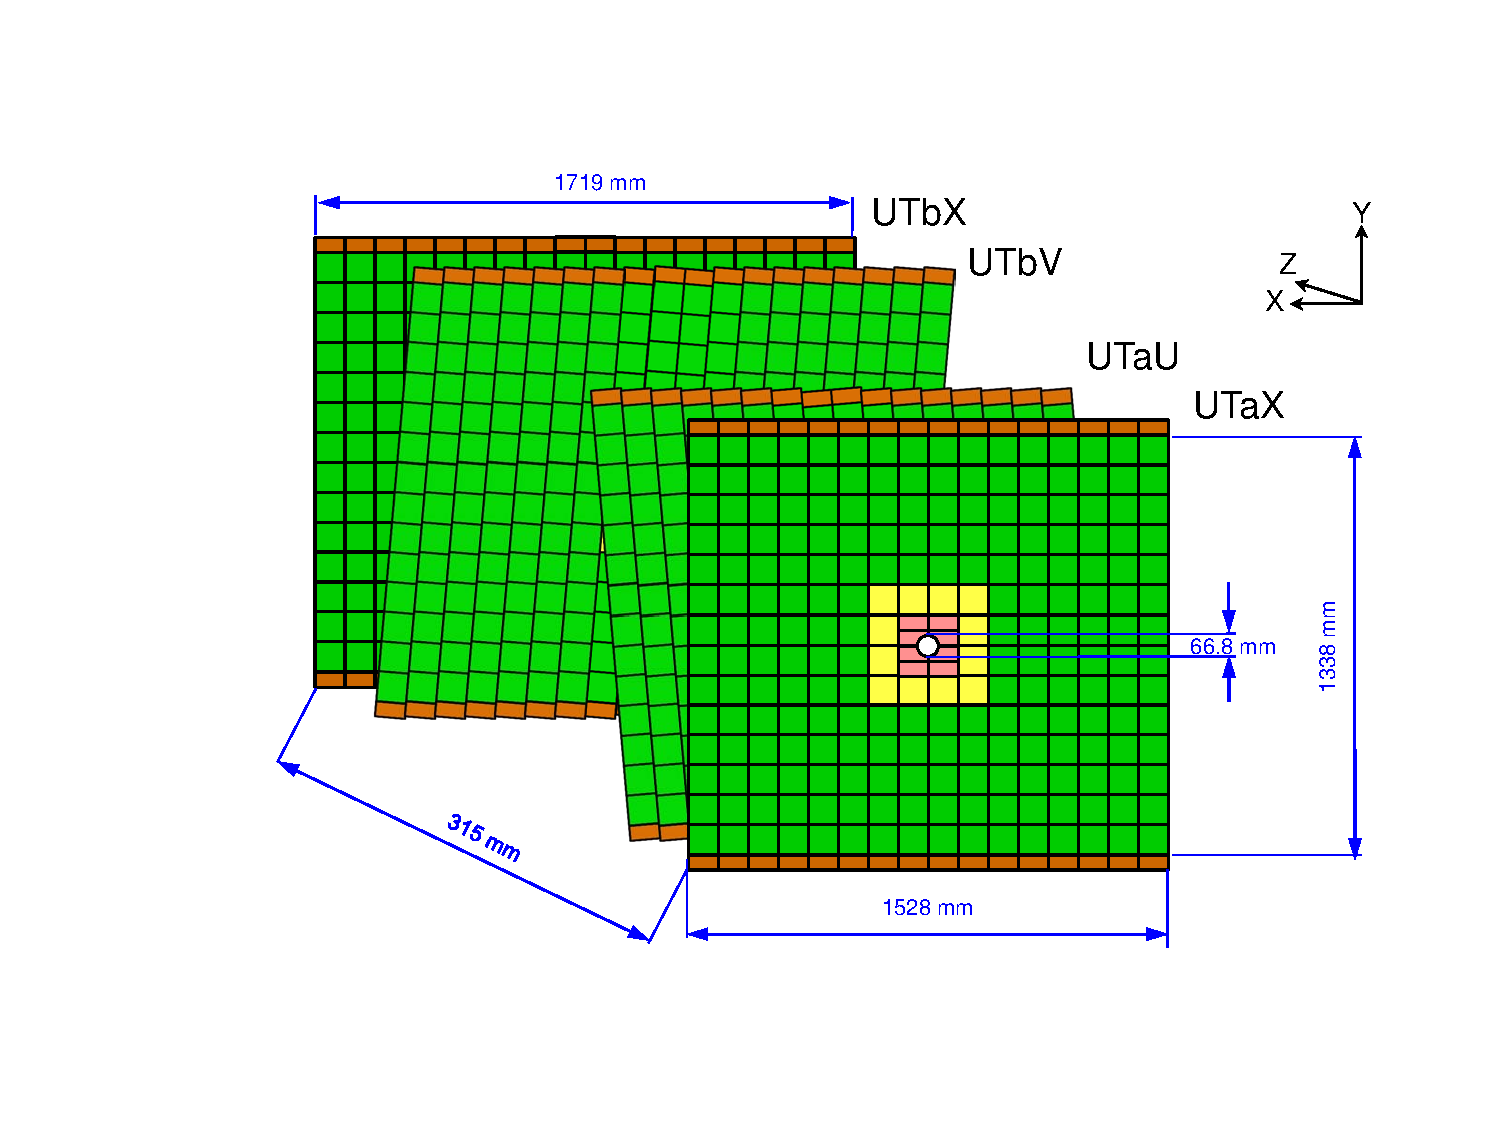
\includegraphics[width=0.8\textwidth]{figs/detector/ut.pdf}
\caption{Schematic view of the UT sub-detector geometry. The different sensor geometries are colour coded.}
\label{fig:ut}
\end{figure}
